\begin{teamsubmission}{Parse-Patrol}{Parse-Patrol: Dual-Mode Chemistry Parsing Infrastructure via MCP Servers}
\authorsblock{
    Nathan Daelman\textsuperscript{1}\orcidlink{0000-0002-7647-1816},
    Christina Ertural\textsuperscript{2}\orcidlink{0000-0002-7696-5824},
    Rubel Mozumber\textsuperscript{1},
    Sascha Klawohn\textsuperscript{1},
    Remya Ann Mathews Kalapurakal\textsuperscript{3} 
}
\affiliationsblock{
    \textsuperscript{1}Humboldt University of Berlin, 10117 Berlin, Germany\\
    \textsuperscript{2}Department of Materials Chemistry, Federal Institute for Materials Research and Testing, 12205 Berlin, Germany\\
    \textsuperscript{3}University of New Hampshire, 03824 Durham, NH, USA
}

\section*{Introduction}

Converting files, oftentimes referred to as \textit{parsing}, is by its very nature dependent on the input and output specifications.
These specifications may exist at a format level, a schema level or more abstractly, an ontological one.
Being dependent on both sides, makes parser infrastructure very brittle and laborintense to maintain.

This is a frequent issue in (materials and chemistry) databases, where results are uploaded in the native specifications of the hardware provider (for experiments), or code maintainer (for computations).
Meanwhile, as database consortia seek to structure these various schemas (and formats) into a more centralized standard, they risk breaking the output specifications of their parsers.
In short, the community needs a robust procedure for rapdily rolling out updates to the standards and schemas down to the infrastructure implementing them.
While the FOSS nature of most scientific projects enables a wide support, the uncoordinated approach of community leaves individual projects vulnerable to source or time cuts.\cite{}  

The more an agent has to rely on itself, rather than its host infrastructure, the more tokens it will consume.

Parse-Patrol combines the best of both worlds, by building off publicly available community parsers and flexibly adapting their output-side via LLM.
It does so via the recently published Model Context Protocol (MCP) framework\cite{mcp}, which has rapidly become an industry standard and is now supported by all major commercial models.
MCP defines a schema in RPC-JSON format for communication between agents and a server that exposes several \textit{components}, listed below.
This specification is both model- and host- (e.g. IDEs, cloud suppliers) agnostic, meaning that it can readily be rolled out to any platform.

\begin{itemize}
  \item software tools.
  \item static and dynamic resources.
  \item specially desgined system prompts.
\end{itemize}

\section*{Results}

When using agentic assistants, the most state-of-the-art mode for running LLMs, there are various pitfalls that may come up:

\begin{itemize}
    \item Few online resources of scientific specifications, or a general lack of documentation.
    \item Long test iteration cycles when programming an implementation from scratch.
\end{itemize}

To circumvent these hurdles we turn to well-established community parsers.
These typically have a more restricted and speciliazed scope for a set of scientific specifications.
Their inclusion enables fast, high-fidelity data extraction and reliable format conversion compare to a standalone agent, while also reducing hallucinations to a minimum.
We provide direct access to these parsers and their documentation via the MCP tools and resources, respectively.
We can then focus on adding support for more parsers to build out a wide coverage, as well as introduce multiple options for the agent to choose from.

Note that MCP does not provide any directives on how to extend the layer in a structured fashion: one by default just extends the list of tools.
Our first technical innovation is thus to define a hiearchical protocol for extending the MCP server.
Each parser is treated as its own MCP server.
This facilitates testing, as the developer can instantiate just that single server.
All MCP components are then automatically registered to the central server, with which the user interacts.
This server should not provide any additional tools of itself.
It predominantly adds its own prompts, which have been engineered to immediately start up the testing phase, given a specification file and some examples.

Where the MCP powers interactive testing and development, actual parsing infrastructure requires code in production.
We observed ourselves that even with access to a MCP parsing server, the agent will without explicit prompting revert back to generating domain-specific parsers from first principles.
These parser prototypes are often erroneous, as the agent cannot generally introspect the MCP server code itself.
Hence, it has no access to how the community parsers are called, or even installed for that matter.

Therefore, we provide the MCP tools, reserved for the exploration phase, as modules\footnote{Depending on the programming community, these may be referred to as \textit{libraries} or \textit{packages}. We use the terminology in Python throughout} too.
These can directly be called from the code.
As modules, we can also guarantee the proper installation setup, further offloading a burden of the agent.

Even so, the agent will not automatically pick up on these modules.
We attribute this behavior to the underlying models not having been trained on a MCP/module hybrid.
Our solution is two-pronged: we provide instructions in the "\\script" prompt to use the modules.
Each parser server exposes its module path and how to call it as a resource.
These are then compiled into a list of resources at the central server detailed above.

Providing such a common solution that is both a MCP sever and a module is not easy.
Each framework has different requirements and is distributed via different channels: MCP Registry\cite{} and PyPi\cite{}, respectively, for example.
Our second innovation, then, is the design of an architecture that supports \textit{dual mode} (cf. Fig.\ref{fig:parse-patrol}), which allows free combination of either feature.
To the best of the authors' knowledge, no other such framework exists that bridges the divide between AI experimentation and production integration.

\begin{figure}[h]
    \centering
    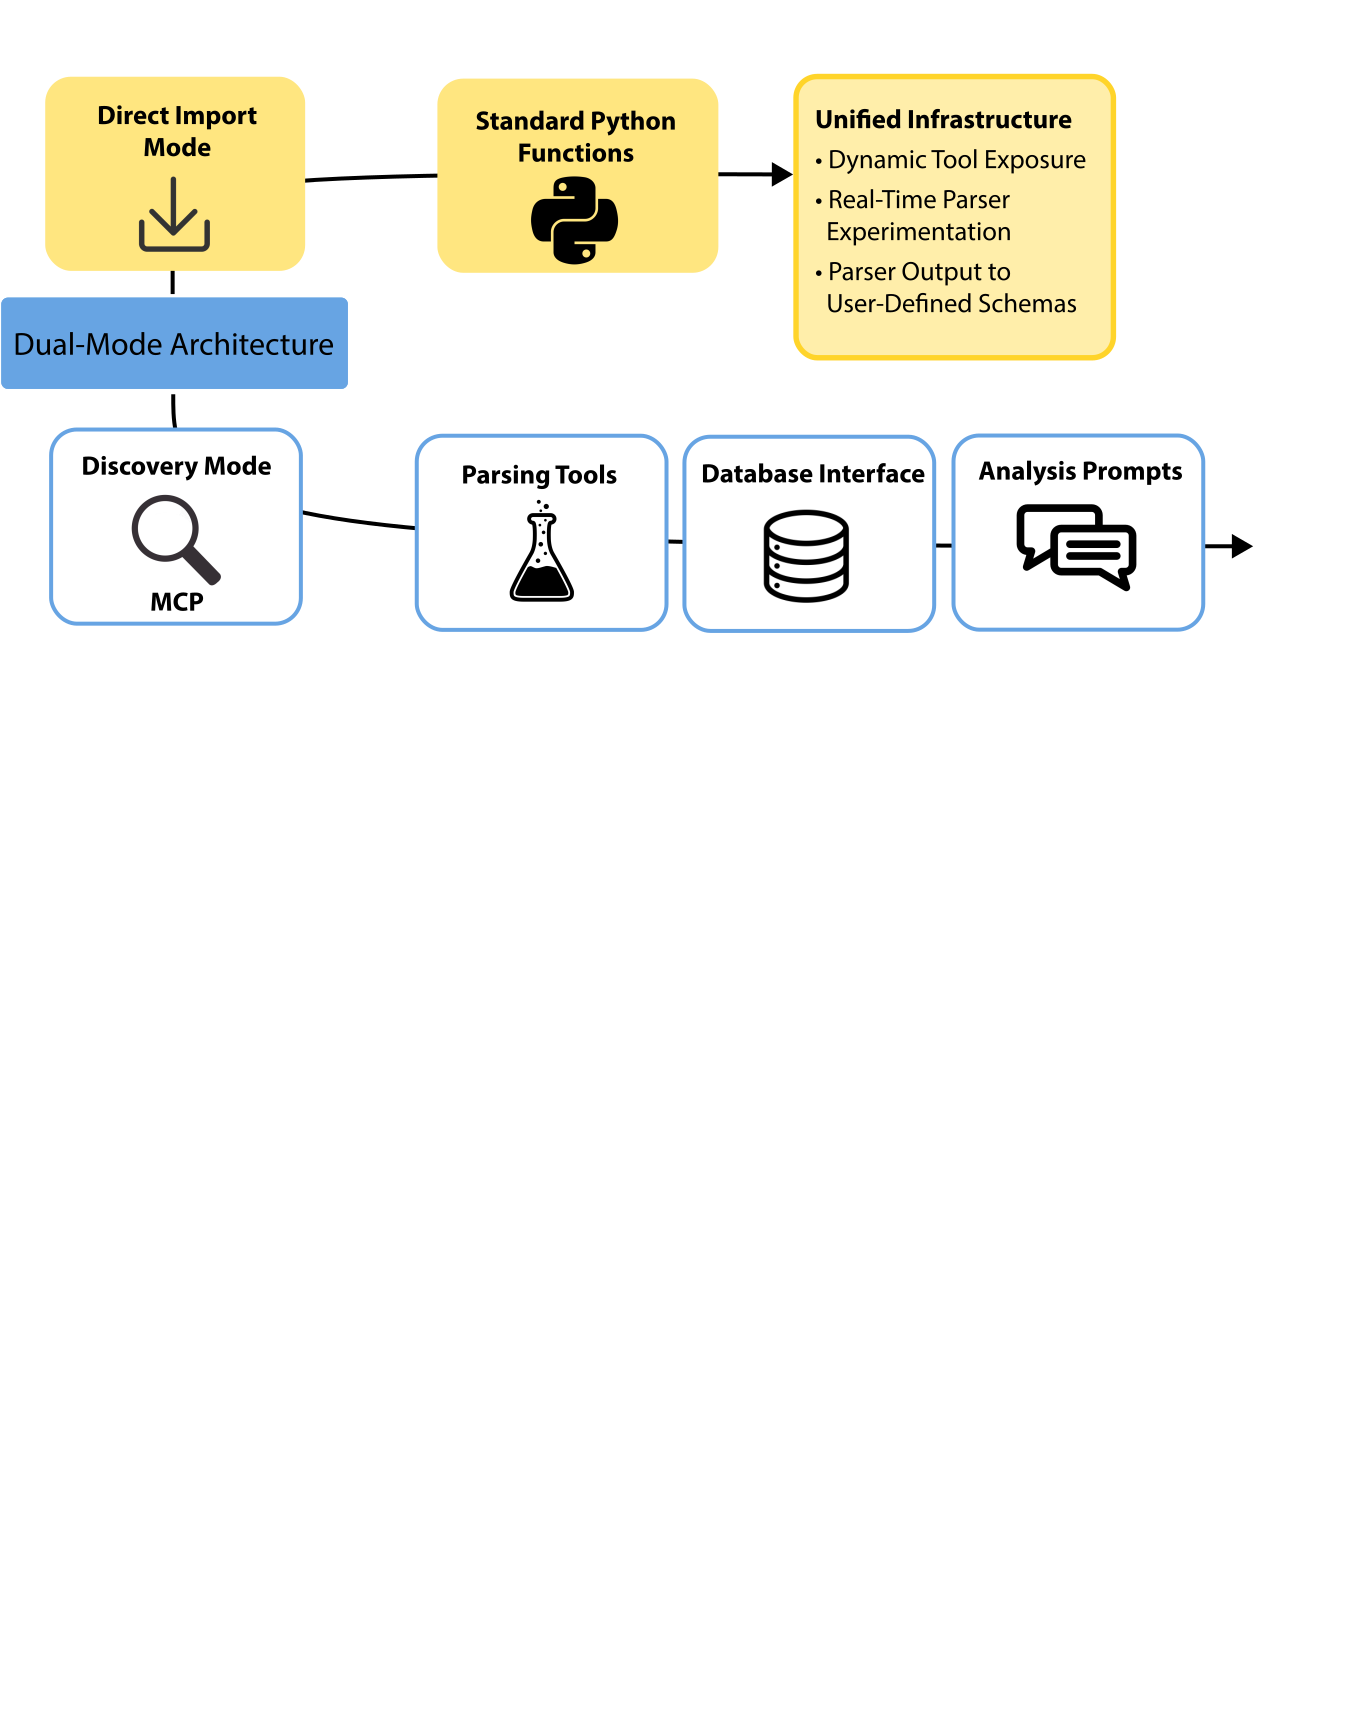
\includegraphics[width=0.5\linewidth]{figures/parse-patrol.png}
    \caption{
    \textbf{Parse-Patrol:}
    The dual-mode architecture allows for user queries via discovery mode and direct Python import mode for parsing big quantum chemistry software files properly.
    }
    \label{fig:parse-patrol}
\end{figure}

\section*{Future Work}

At the time of writing, the repository is seeing active development.
Recent additions include a streamlining of the architecture and file structure.:
Given the well-defined objective of providing a computational parsers toolkit, future extensions are not excluded.
This project is under consideration for incorporation into NOMAD\cite{nomad_lab,draxl2019nomad} parser suite.

\section*{Open-source Materials}

The open-source code is available on GitHub: \github{https://github.com/ndaelman-hu/parse-patrol}. 
A demo video is available on YouTube: \youtube{https://www.youtube.com/watch?v=fSAyi5ubkR0}.

\section*{Author Contributions}

\textbf{N.D.}: Conceptualization, Software, Original Code Draft, Visualization, Writing - Editing,
\textbf{C.E.}: Conceptualization Revision, Software, Visualization, Video Editing, Writing - Original Manuscript Text Draft, Figure, Editing
\textbf{R.M.}: Implementation asynchronous servers, Extension Testing Infrastructure - Conceptualization Revision 
\textbf{S.K.}: Rollout Parser Support 

\section*{Acknowledgements}
The authors thank for their financial support the NFDI consortium FAIRmat, funded by the German Research Foundation (DFG, Deutsche Forschungsgemeinschaft) in project 460197019.

\end{teamsubmission}
